\documentclass
[handout]
{beamer}
\documentclass{beamer}

%%
%%
%%
% From http://tex.stackexchange.com/questions/2072/beamer-navigation-circles-without-subsections
% Solution #2 or 3:
% \usepackage{etoolbox}
% \makeatletter
% % replace the subsection number test with a test that always returns true
% \patchcmd{\slideentry}{\ifnum#2>0}{\ifnum2>0}{}{\@error{unable to patch}}%
% \makeatother
% Solution #1:
\usepackage{remreset}% tiny package containing just the \@removefromreset command
\makeatletter
\@removefromreset{subsection}{section}
\makeatother
\setcounter{subsection}{1}


\usepackage{etex}
\usepackage{pgf}
\usepackage{tikz}
\usepackage{url}
\usepackage{amsmath}
\usepackage{color}
% \definecolor{red}{rgb}{1,0,0}
\usepackage{ulem}
% \usepackage{booktabs}
\usepackage{colortbl,booktabs}
\renewcommand*{\thefootnote}{\fnsymbol{footnote}}
\usepackage{fancybox}
\usepackage[framemethod=TikZ]{mdframed}
\mdfdefinestyle{FactStyle}{%
  outerlinewidth=0.5,
  roundcorner=1pt,
  leftmargin=1cm,
  linecolor=blue,
  outerlinecolor=blue!70!black,
  backgroundcolor=yellow!40
}
\usepackage{cancel}

  \newcommand\Warning{%
    \makebox[2.4em][c]{%
      \makebox[0pt][c]{\raisebox{.2em}{\Large!}}%
      \makebox[0pt][c]{\color{red}\Huge$\bigtriangleup$}}}%

\usepackage{stackengine}
\usepackage{scalerel}
\usepackage{xcolor}
  \newcommand\dangersign[1][2ex]{%
    \renewcommand\stacktype{L}%
    \scaleto{\stackon[1.3pt]{\color{red}$\triangle$}{\tiny !}}{#1}%
  }



\usepackage{dcolumn}
\newcolumntype{d}[1]{D{.}{.}{#1}}

% From
% http://tex.stackexchange.com/questions/109900/how-can-i-box-multiple-aligned-equations
\usepackage{empheq}
\usepackage{tcolorbox}  \newtcbox{\othermathbox}[1][]{%
  nobeforeafter, tcbox raise base, 
  colback=black!10, colframe=red!30, 
  left=1em, top=0.5em, right=1em, bottom=0.5em}

\newcommand\blue{\color{blue}}
\newcommand\red{\color{red}}
\newcommand\green{\color{green!75!black}}
\newcommand\purple{\color{purple}}
\newcommand\bluegreen{\color{blue!75!green}}
\newcommand\orange{\color{orange}}
\newcommand\redgreen{\color{red!50!green}}
\newcommand\grey{\color{black}}
\newcommand\gap{\vspace{.1in}}
\newcommand\nb{${\red\bullet}\ $}
\newcommand\halfgap{\vspace{.05in}}
\newcommand\divideline{\line(1,0){352}}
\usepackage{marvosym} % for \Smiley

\newcommand{\bluealert}[1]{{\blue\textbf{#1}}}

% \usepackage{beamerthemesplit} %Key package for beamer
\usetheme{Singapore}
% \usetheme{Szeged}
% \usetheme{Garfield}
% \usetheme{CambridgeUS}
% \usenavigationsymbolstemplate{} %Gets rid of slide navigation symbols


\setbeamercolor{separation line}{use=structure,bg=structure.fg!50!bg}
% \begin{beamercolorbox}[colsep=0.5pt]
%   {upper separation line foot}
% \end{beamercolorbox}



\makeatletter
\setbeamertemplate{footline}
{
  \leavevmode%
  \hbox{%
% \begin{beamercolorbox}[colsep=0.5pt]
%   {upper separation line foot}
% \end{beamercolorbox}


  \begin{beamercolorbox}[wd=.5\paperwidth,ht=2.25ex,dp=2ex,colsep=0.5pt]%
    {upper separation line foot}
    \usebeamerfont{author in head/foot}%
    \hspace*{2ex}\insertshortdate:\ \insertshorttitle
  \end{beamercolorbox}%
  \begin{beamercolorbox}[wd=.5\paperwidth,ht=2.25ex,dp=2ex,right]{title in head/foot}%
    \usebeamerfont{title in head/foot}
    {\insertshortauthor}\hspace*{2ex}
  \end{beamercolorbox}}%
  % \begin{beamercolorbox}[wd=.333333\paperwidth,ht=2.25ex,dp=2ex,right]{date in head/foot}%
  %   \usebeamerfont{date in head/foot}\insertshortdate{}\hspace*{2em}
  %   \insertframenumber{} / \inserttotalframenumber\hspace*{2ex} 
  % \end{beamercolorbox}%
  \vskip0pt%
}
\makeatother

\usetikzlibrary{decorations.markings}
\usetikzlibrary{arrows}


\title{Final Exam Review}
\author{Peter Garfield, UCSB Mathematics}
\date{March 15, 2017}
%\institute{}


\useinnertheme{default}

\usefonttheme{serif}
% \usecolortheme{rose}
% \usecolortheme{whale}
% \usecolortheme{orchid}
\usecolortheme{crane}
% \usecolortheme{dolphin}


%TEMPLATE
\setbeamertemplate{navigation symbols}{}

\setbeamertemplate{note page}[compress]

\setbeamertemplate{frametitle}{
  \vspace{0.5em}
  % \begin{centering}
  {\huge\blue\textbf{\textmd{\insertframetitle}}}
  \par
  % \end{centering}
}

% From http://tex.stackexchange.com/questions/7032/good-way-to-make-textcircled-numbers:
\newcommand*\circled[1]{\tikz[baseline=(char.base)]{\node[shape=circle,draw,fill=orange,inner sep=1pt] (char) {#1};}} 
% \renewcommand{\labelenumi}{\circled{\textbf{\arabic{enumi}}}}

\let\olddescription\description
\let\oldenddescription\enddescription
\usepackage{enumitem}
\let\description\olddescription
\let\enddescription\oldenddescription

% \usepackage[loadonly]{enumitem}
\setlist[enumerate,1]{label=\colorbox{orange}{\arabic*.},font=\bfseries}
%\setlist[enumerate,2]{label=\colorbox{blue!25}{(\alph*)},font=\bfseries}
% \setlist[enumerate,1]{label=\arabic*.,font=\bfseries}
\setlist[itemize,1]{label=\red$\bullet$}
\setlist[itemize,2]{label=\blue$\bullet$}

\newcommand\answer[1]{\fbox{#1}}
% \renewcommand\answer[1]{}

\newcommand{\antilog}{\operatorname{antilog}}








\title{}
\title{Calculus Intro}
\date{May 24, 2022}


\begin{document}
\small



\frame{
  \frametitle{}
    {\Huge{}Welcome Back!}\\[.5em]

  {\Huge{}Differential Calculus}
  \vfill
  {\Large{}Instructor:}\\
  \ \hspace*{0.2in} \instructor
  
   \url{schley@math.ucsb.edu}\\
  \ \hspace*{0.2in} \officeloc
  \\[0.5em]

  {\Large{}Office Hours:}\\
  \ \hspace*{0.2in} \officehours 
  \bigskip

  \copyright\ 2022\ Daryl Cooper, Peter M.\ Garfield, Ebrahim Ebrahim \& Nathan Schley\\
  Please do not distribute outside of this course.
  \vfill

}











\section*{Review}

\frame{
A nice thing about derivatives...
\begin{align*}  
\frac{d}{dx} ( a\cdot f(x) + b\cdot g(x) ) 
&= a\frac{d}{dx}f(x) + b\frac{d}{dx} g(x)\\[0.75em]
&= a\cdot f'(x)+b\cdot g'(x)
\end{align*}
For example...
\pause
$$
\begin{array}{lclcl}
 \frac{d}{dx} ( 3x^2+ 5x ) &=& 3  \frac{d}{dx} x^2 &+ & 5 \frac{d}{dx}x\\[0.75em]
                           &=& 3(2x)               &+  & 5(1)\\[0.75em]
                           &=& 6x                  &+ & 5
\end{array}
$$
}


\frame{
  \frametitle{A Warning!}

  \begin{empheq}[box=\othermathbox]{align*}
    \ \hfill \raisebox{-0.5em}{\dangersign[6ex]} \hspace*{0.2in}
    \frac{d}{dx}\left(f(x)g(x)\right) {\red\ne} f'(x) \times g'(x)
    \hspace*{0.2in} \raisebox{-0.5em}{\dangersign[6ex]} \hfill \ 
  \end{empheq}
  \pause
  \bigskip

  \alert{Example:} What is the derivative of $(x^3+1)(2x^2-3x+5)$?
  \bigskip
  \pause

  \alert{Question:}\ $\displaystyle\frac{d}{dx}\left((x^3+1)(2x^2-3x+5)\right)=$? \\ 
  \begin{center}
    A$=10x^4-8x^3+10x^2+12x-3$
    \quad 
    B$ = 10x^4-12x^3+15x^2+4x+5$
    \\ \\ 
    C$ = 10x^4-12x^3+15x^2+4x-3$
    \quad 
    D$ = \text{Other}$
  \end{center}
  \bigskip
  \pause
  {\blue Hint: $2x^5 -3x^4 + 5x^3 + 2x^2 - 3x + 6$}
  \bigskip
  \pause
  
  \alert{Answer:}\ \fbox{C}

  \vspace*{2in}

}





\frame{
  \frametitle{Differentiating $f(x) = e^{kx}$}

  \begin{minipage}[b]{0.35\linewidth}
    \begin{empheq}[box=\othermathbox]{align*}
      \frac{d}{dx}\left(e^{{\red k}x}\right) 
      & = {\red k}e^{{\red k}x}
    \end{empheq}
  \end{minipage}
  \hspace*{0.2in}
  versus
  \hspace*{0.2in}
  \begin{minipage}[b]{0.35\linewidth}
    \begin{empheq}[box=\othermathbox]{align*}
      \frac{d}{dx}\left(x^{{\red n}}\right) 
      & = {\red n} x^{{\red n}-1}
    \end{empheq}
  \end{minipage}
  \bigskip

  \begin{empheq}[box=\othermathbox]{align*}
    \raisebox{-0.5em}{\dangersign[6ex]}  
    \hspace*{0.1in}
    \text{These are not polynomials. }\ 
    \dfrac{d}{dx} \big( e^{{\red k}x} \big) \neq {\red k}e^{({\red k}-1)x}.
    \hspace*{0.1in}
    \raisebox{-0.5em}{\dangersign[6ex]}  
  \end{empheq}
  \bigskip

  \alert{Question:}\ Find $\dfrac{d}{dx}\left( 4e^{3x}+ 5x^3\right)$
  \begin{center}
    A$=12e^{2x}+15x^2$
    \qquad 
    B$ = 12e^{3x}+15 x^3$
    \qquad 
    C$ = 4e^{3x}+15x^2$
    \\
    \ 
    \quad 
    D$=12e^{3x}+15x^2$
    \quad
    E$= \text{Other}$
    \pause
    \quad
    \fbox{D}
  \end{center}

}




\frame{
  \frametitle{Meanings: The First Derivative}

  \begin{center}
    \begin{tikzpicture}[x=15mm,y=5mm,>=latex]
      \only<1>{%
        \draw[ultra thick,blue,domain=-1:3,smooth] plot (\x,{(\x)^3-3*(\x)^2+2});
      }
      \only<2->{%
        \draw[ultra thick,blue,domain=-1:0,smooth] plot (\x,{(\x)^3-3*(\x)^2+2});
        \draw[ultra thick,red,domain=0:2,smooth] plot (\x,{(\x)^3-3*(\x)^2+2});
        \draw[ultra thick,blue,domain=2:3,smooth] plot (\x,{(\x)^3-3*(\x)^2+2});
        \filldraw[green] (0,2) circle (2pt);
        \filldraw[green] (2,-2) circle (2pt);
      }
      \uncover<3->{%
        \draw[ultra thick,blue,<-] (-1,-2.5) -- (0,-2.5);
        \draw[blue,fill=white] (0,-2.5) circle (2pt);
        \draw[ultra thick,blue,->] (2,-2.5) -- (3,-2.5);
        \draw[blue,fill=white] (2,-2.5) circle (2pt);
        \draw[ultra thick,red] (0,-2.85) -- (2,-2.85);
        \draw[red,fill=white] (0,-2.85) circle (2pt);
        \draw[red,fill=white] (2,-2.85) circle (2pt);
        \node[blue] at (-0.5,-3.5) {$f(x)$ incr};
        \node[red] at (1,-3.5) {$f(x)$\ decr};
        \node[blue] at (2.5,-3.5) {$f(x)$\ incr};
      }
      \uncover<5->{%
        \node[blue] at (-0.5,-4.5) {$f'(x)>0$};
        \node[red] at (1,-4.5) {$f'(x)<0$};
        \node[blue] at (2.5,-4.5) {$f'(x)>0$};
      }
      \begin{scope}
        \clip (-1.5,-4) rectangle (3.5,2.75);
              \uncover<4->{%
        % Tangent lines to $y=x^3-3x^2+2$ has slope $y'=3x^2-6x=3x(x-2)$.
        % \draw[blue,domain=-1:0] plot (\x,{(-5/5)^3-3*(-5/5)^2+2+3*(-5/5)*(-5/5-2)*(\x+5/5)});
        % \draw[blue,domain=-1:0] plot (\x,{(-4/5)^3-3*(-4/5)^2+2+3*(-4/5)*(-4/5-2)*(\x+4/5)});
        % \draw[blue,domain=-1:0] plot (\x,{(-3/5)^3-3*(-3/5)^2+2+3*(-3/5)*(-3/5-2)*(\x+3/5)});
        % \draw[blue,domain=-1:0] plot (\x,{(-2/5)^3-3*(-1/5)^2+2+3*(-2/5)*(-2/5-2)*(\x+2/5)});
        % \draw[blue,domain=-1:0] plot (\x,{(-1/5)^3-3*(-1/5)^2+2+3*(-2/5)*(-1/5-2)*(\x+1/5)});
        % \draw[blue,domain=-1:0] plot (\x,{(-1/3)^3-3*(-1/3)^2+2+3*(-1/3)*(-1/3-2)*(\x+1/3)});
        \draw[thick,blue,domain=-1:0] plot (\x,{(-1/2)^3-3*(-1/2)^2+2+3*(-1/2)*(-1/2-2)*(\x+1/2)});
        \draw[thick,red,domain=0:1.85] plot (\x,{(1)^3-3*(1)^2+2+3*(1)*(1-2)*(\x-1)});
        \draw[thick,blue,domain=2.2:3.5] plot (\x,{(2.5)^3-3*(2.5)^2+2+3*(2.5)*(2.5-2)*(\x-2.5)});
        \fill[black] (-0.5,{(-1/2)^3-3*(-1/2)^2+2}) circle (2pt);
        \fill[black] (1,{(1)^3-3*(1)^2+2}) circle (2pt);
        \fill[black] (2.5,{(2.5)^3-3*(2.5)^2+2}) circle (2pt);
      }
      \end{scope}
    \end{tikzpicture}
  \end{center}
  \bigskip

  \uncover<6->{%
    \bluealert{Point:} 

    \begin{mdframed}[style=FactStyle]
      \vspace*{-1.25em}
      \begin{align*}
        {\blue f'(x) > 0} & \iff\ \text{$f(x)$\ is increasing} \\
        {\red f'(x) < 0} & \iff\ \text{$f(x)$\ is decreasing} 
      \end{align*}
    \end{mdframed}
  }
  \vspace*{3in}

}

\frame{
  \frametitle{Meanings: The Second Derivative}

  \begin{center}
    \begin{tikzpicture}[x=15mm,y=5mm,>=latex]
      \only<1>{%
        \draw[ultra thick,blue,domain=-1:3,smooth] plot (\x,{(\x)^3-3*(\x)^2+2});
      }
      \only<2->{%
        \draw[ultra thick,green!50!black,domain=-1:1,smooth] plot (\x,{(\x)^3-3*(\x)^2+2});
        \draw[ultra thick,orange!90!black,domain=1:3,smooth] plot (\x,{(\x)^3-3*(\x)^2+2});
        \filldraw[blue] (1,0) circle (2pt);
      }
      \uncover<3->{%
        \draw[ultra thick,green!50!black,<-] (-1,-2.5) -- (1,-2.5);
        \draw[green!50!black,fill=white] (1,-2.5) circle (2pt);
        \draw[ultra thick,orange!90!black,->] (1,-2.85) -- (3,-2.85);
        \draw[orange!90!black,fill=white] (1,-2.85) circle (2pt);
        \node[green!50!black] at (0,-3.5) {$f(x)$ cc down};
        \node[orange!90!black] at (2,-3.5) {$f(x)$\ cc up};
      }
      \begin{scope}
        \clip (-1.5,-4) rectangle (3.5,2.75);
              \uncover<4->{%
        % Tangent lines to $y=x^3-3x^2+2$ has slope $y'=3x^2-6x=3x(x-2)$.
        % \draw[blue,domain=-1:0] plot (\x,{(-5/5)^3-3*(-5/5)^2+2+3*(-5/5)*(-5/5-2)*(\x+5/5)});
        % \draw[blue,domain=-1:0] plot (\x,{(-4/5)^3-3*(-4/5)^2+2+3*(-4/5)*(-4/5-2)*(\x+4/5)});
        % \draw[blue,domain=-1:0] plot (\x,{(-3/5)^3-3*(-3/5)^2+2+3*(-3/5)*(-3/5-2)*(\x+3/5)});
        % \draw[blue,domain=-1:0] plot (\x,{(-2/5)^3-3*(-1/5)^2+2+3*(-2/5)*(-2/5-2)*(\x+2/5)});
        % \draw[blue,domain=-1:0] plot (\x,{(-1/5)^3-3*(-1/5)^2+2+3*(-2/5)*(-1/5-2)*(\x+1/5)});
        % \draw[blue,domain=-1:0] plot (\x,{(-1/3)^3-3*(-1/3)^2+2+3*(-1/3)*(-1/3-2)*(\x+1/3)});
        \draw[thick,green!50!black,domain=-1:0] plot (\x,{(-2/3)^3-3*(-2/3)^2+2+3*(-2/3)*(-2/3-2)*(\x+2/3)});
        \draw[thick,green!50!black,domain=-1:0.3333] plot (\x,{(-1/3)^3-3*(-1/3)^2+2+3*(-1/3)*(-1/3-2)*(\x+1/3)});
        \draw[thick,green!50!black] (-0.5,2) -- (0.5,2);
        \draw[thick,green!50!black,domain=-0.3333:1] plot (\x,{(1/3)^3-3*(1/3)^2+2+3*(1/3)*(1/3-2)*(\x-1/3)});
        \draw[thick,green!50!black,domain=0:1] plot (\x,{(2/3)^3-3*(2/3)^2+2+3*(2/3)*(2/3-2)*(\x-2/3)});
        % \draw[thick,red,domain=0:1.85] plot (\x,{(1)^3-3*(1)^2+2+3*(1)*(1-2)*(\x-1)});
        % \draw[thick,blue,domain=2.2:3.5] plot (\x,{(2.5)^3-3*(2.5)^2+2+3*(2.5)*(2.5-2)*(\x-2.5)});
        \fill[black] ({-2/3},{(-2/3)^3-3*(-2/3)^2+2}) circle (2pt);
        \fill[black] ({-1/3},{(-1/3)^3-3*(-1/3)^2+2}) circle (2pt);
        \fill[black] (0,2) circle (2pt);
        \fill[black] ({1/3},{(1/3)^3-3*(1/3)^2+2}) circle (2pt);
        \fill[black] ({2/3},{(2/3)^3-3*(2/3)^2+2}) circle (2pt);
        % \fill[black] (1,{(1)^3-3*(1)^2+2}) circle (2pt);
        % \fill[black] (2.5,{(2.5)^3-3*(2.5)^2+2}) circle (2pt);
      }
      \uncover<6->{%
        \draw[thick,orange!90!black,domain=2.3:3.3] plot (\x,{(8/3)^3-3*(8/3)^2+2+3*(8/3)*(8/3-2)*(\x-8/3)});
        \draw[thick,orange!90!black,domain=1.9:2.9] plot (\x,{(7/3)^3-3*(7/3)^2+2+3*(7/3)*(7/3-2)*(\x-7/3)});
        \draw[thick,orange!90!black] (1.5,-2) -- (2.5,-2);
        \draw[thick,orange!90!black,domain=1.3333:2.1] plot (\x,{(5/3)^3-3*(5/3)^2+2+3*(5/3)*(5/3-2)*(\x-5/3)});
        \draw[thick,orange!90!black,domain=0.5:2] plot (\x,{(4/3)^3-3*(4/3)^2+2+3*(4/3)*(4/3-2)*(\x-4/3)});
        % \draw[thick,red,domain=0:1.85] plot (\x,{(1)^3-3*(1)^2+2+3*(1)*(1-2)*(\x-1)});
        % \draw[thick,blue,domain=2.2:3.5] plot (\x,{(2.5)^3-3*(2.5)^2+2+3*(2.5)*(2.5-2)*(\x-2.5)});
        \fill[black] ({4/3},{(4/3)^3-3*(4/3)^2+2}) circle (2pt);
        \fill[black] ({5/3},{(5/3)^3-3*(5/3)^2+2}) circle (2pt);
        \fill[black] (2,-2) circle (2pt);
        \fill[black] ({7/3},{(7/3)^3-3*(7/3)^2+2}) circle (2pt);
        \fill[black] ({8/3},{(8/3)^3-3*(8/3)^2+2}) circle (2pt);
      }
      \end{scope}
      \uncover<5->{%
        \node[green!50!black] at (0,-4.5) {$f''(x)<0$};
      }
      \uncover<7->{%
        \node[orange!90!black] at (2,-4.5) {$f''(x)>0$};
      }
    \end{tikzpicture}
  \end{center}
  \vspace*{-1em}

  \uncover<8->{%
    \bluealert{Point:} 

    \begin{mdframed}[style=FactStyle]
      \vspace*{-1.25em}
      \begin{align*}
        {\color{orange!90!black}f''(x) > 0} 
        & \iff\ \text{$f'(x)$\ is increasing} \\
        & \iff\ \text{$f(x)$\ is concave up} \\[0.5em]
        {\color{green!50!black}f''(x) < 0}
        & \iff\ \text{$f'(x)$\ is decreasing} \\
        & \iff\ \text{$f(x)$\ is concave down} 
      \end{align*}
    \end{mdframed}
  }
  \vspace*{3in}

}



\frame{
  \frametitle{Concavity}

  \begin{mdframed}[style=FactStyle]
    \vspace*{-1.25em}
    \begin{align*}
      {\color{orange!90!black}f''(x) > 0} & \iff\ \text{$f(x)$\ is concave up} \\
      {\color{green!50!black}f''(x) < 0} & \iff\ \text{$f(x)$\ is concave down} 
    \end{align*}
  \end{mdframed}

  {\red(1)}\ For which values of $x$ is $f(x)=x^3-6x^2+3x+2$ concave up?
  \begin{center}
    A\ when $x=0$
    \quad 
    B\ when $x<6$
    \quad 
    C\ when $x>6$\\
    \ 
    \quad 
    D\ when $x<2$
    \quad 
    E\ when $x>2$
    \quad
    \uncover<2->{\fbox{E}}
  \end{center}

  \uncover<3->{
  {\red(2)}\ Where is $f{\red''}(x)>0$? 

  \
  \hfill
  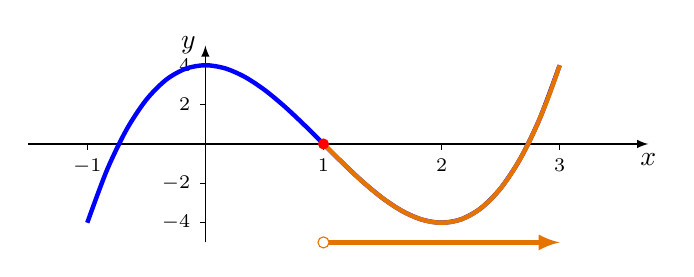
\begin{tikzpicture}[x=15mm,y=2.5mm,>=latex]
    %
    \draw[thin,black,->] (-1.5,0) -- (3.75,0) node[below] {$x$};
    \draw[thin,black,->] (0,-5) -- (0,5) node[left] {$y$};
    % ticks:
    \foreach \x in {-1,1,2,3}
    {
      \draw[thin,black] (\x,0) -- (\x,-2pt) node[below] {$\scriptstyle\x$};
    }
    \foreach \y in {-4,-2,2,4}
    {
      \draw[thin,black] (0,\y) -- (-2pt,\y) node[left] {$\scriptstyle\y$};
    }
    \draw[ultra thick,blue,domain=-1:3,smooth] plot (\x,{2*(\x)^3-6*(\x)^2+4});
    \uncover<4->{%
      \draw[ultra thick,orange!90!black,domain=1:3,smooth] plot (\x,{2*(\x)^3-6*(\x)^2+4});
      \draw[ultra thick,orange!90!black,->] (1,-5) -- (3,-5);
      \draw[orange!90!black,fill=white] (1,-5) circle (2pt);
      \fill[red] (1,0) circle (2pt);
    }
  \end{tikzpicture}
  \hfill
  \ 
  \vspace*{-1em}

  \begin{center}
    A\ when $x<2$
    \quad 
    B\ when $x>2$
    \quad
    C\ when $x<1$\\
    \ 
    \quad 
    D\ when $x>1$
    \quad
    E\ when $-0.7<x<1$
    \pause
    \quad
    \uncover<4->{\fbox{D}}
  \end{center}
}

}


\if0
\frame{
  \frametitle{Review:}

  {\red(1)}\ Where is  $f(x)=3x^2+18x-4$ increasing?
  \begin{center}
    A\ $x < -3$
    \quad 
    B\ $x > -3$
    \quad 
    C\ $x < 3$
    \quad 
    D\ $x > 3$
    \quad 
    E\ $x=3$
    \quad
    \pause
    \fbox{B}
  \end{center}
  \bigskip

  {\red(2)}\ Where is $f(x)$ increasing?
  \begin{center}
    \includegraphics[scale=0.7]{Figures/concave4.pdf}
  \end{center}
  \begin{center}
    A\ $x<0$
    \quad 
    B\ $x>2$
    \quad
    C\ $x<2$
    \quad 
    D\ $0<x<2$
    \quad
    E\ $x>0$
    \quad
    \pause
    \fbox{D}
  \end{center}
  
}

\frame{
  \frametitle{Continuing Review}

  \begin{center}
    \only<1-4>{\includegraphics[scale=0.7]{Figures/concave4.pdf}}
    \only<5->{\includegraphics[scale=0.7]{Figures/concave5.pdf}}
  \end{center}

  {\red(3)} Where is $f''(x)<0$?
  \begin{center}
    A\ $1<x<3$
    \quad 
    B\  $x>3$
    \quad 
    C\ $x>2$
    \quad 
    D\ $0<x<2$
    \quad 
    E\ $x<1$
    \quad
    \uncover<2->{\fbox{A}}
  \end{center}
  \bigskip

  \uncover<3->{%
  {\red(4)}\ Where is $f'(x)$ decreasing?
  \begin{center}
    A\ $1<x<3$
    \quad 
    B\  $x>3$
    \quad 
    C\ $x>2$
    \quad 
    D\ $0<x<2$
    \quad 
    E\ $x<1$
    \pause
    \quad
    \uncover<4->{\fbox{A}}
  \end{center}
  }
  \bigskip

  % {\red(5)}\ Where is $f(x)$ concave down?
  % \begin{center}
  %   A\ $1<x<3$
  %   \quad 
  %   B\  $x>3$
  %   \quad 
  %   C\ $x>2$
  %   \quad 
  %   D\ $0<x<2$
  %   \quad 
  %   E\ $x<1$
  %   \pause
  %   \quad
  %   \fbox{A}
  % \end{center}
  % \bigskip

}


\frame{
  \frametitle{Which Company Is Better?}

  \begin{center}
    \includegraphics[scale=1]{Figures/companyAB.pdf}
  \end{center}

  \alert{Question:}\ Which company, A or B, would you invest in?
  \pause 

  \begin{itemize}
  \item[\nb] During this time period, {\red A has made
      smaller profits than B}.

  \item[\nb] But it {\blue looks like} A will do better in the future.
  \item[\nb] Why? \pause The concavity! Getting {\blue better}\ or getting {\blue worse}.
    \pause
  \item[\nb] For profit we want concave up. But for the spread of an infectious disease we want concave down.
  \end{itemize}


}
\fi

\section{Optimization}
\frame{
  \frametitle{\S8.13: Max/Min problems}

  Often want to find the biggest, smallest, most, least, maximum, minimum of something.

  \begin{minipage}{0.4\linewidth}
    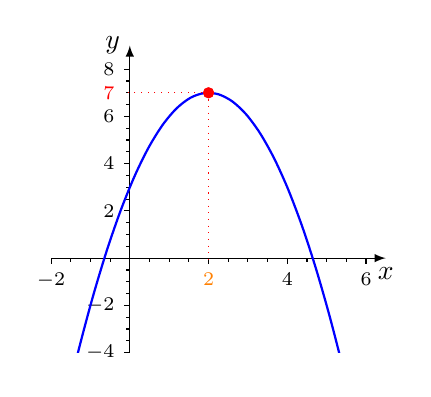
\begin{tikzpicture}[x=5mm,y=3mm,>=latex]
      \draw[thin,black,->] (-2,0) -- (6.5,0) node[below] {$x$};
      \draw[thin,black,->] (0,-4) -- (0,9) node[left] {$y$};
      % ticks:
      \foreach \x in {-2,2,4,6}
      {
        \draw[thin,black] (\x,0) -- (\x,-2pt) node[below] {$\scriptstyle\x$};
      }
      \foreach \x in {-2,-1.5,...,6.2}
      {
        \draw[thin,black] (\x,0) -- (\x,-1.5pt);
      }
      \foreach \y in {-4,-2,2,4,6,8}
      {
        \draw[thin,black] (0,\y) -- (-2pt,\y) node[left] {$\scriptstyle\y$};
      }
      \foreach \y in {-4,-3.5,...,8.2}
      {
        \draw[thin,black] (0,\y) -- (-1.5pt,\y);
      }
      \begin{scope}
        \clip (-2,-4) rectangle (6,8);
        \draw[thick,blue,domain=-2:6.5,smooth] plot (\x,{-1*(\x)^2+4*\x+3});
      \end{scope}
      \uncover<2->{%
        \draw[thin,red,dotted] (2,7) -- (-2pt,7) node[left] {$\scriptstyle7$};
        \fill[red] (2,7) circle (2pt);
      }
      \uncover<3->{%
        \draw[thin,red,dotted] (2,7) -- (2,-2pt) node[below,orange,fill=white] {$\scriptstyle2$};
        \fill[red] (2,7) circle (2pt);
      }
    \end{tikzpicture}
  \end{minipage}
  \hspace*{0.25in}
  \parbox{50mm}{%
    Here's the graph of \\
    $y = f(x)=-x^2+4x+3$
    \gap

    \uncover<2->{%
      The \emph{maximum value} or just \emph{maximum} of the function is ${\red 7}.$ 
    }
    \gap

    \uncover<3->{
      The \emph{value of $x$}\ which gives the maximum of $f(x)$ is $x={\orange 2}$
    }
    \gap

    \uncover<4->{%
      We write ${\blue f({\orange 2})} = {\red 7}$.
    }
  }
  \gap

  \uncover<5->{%
    For this example you can see this is the maximum because
    \begin{equation*}
      f(x) 
      = -x^2+4x+3
      = -(x-{\orange 2})^2+{\red 7}
    \end{equation*}
    $(x-{\orange 2})^2$ is always positive except when $x=\orange 2$\\
    {\blue so the maximum  must} be at $x=\orange 2$. \pause {\red But there is an easier way.}
  }

}

\frame{
  \frametitle{How To Find A Maximum}

  \begin{mdframed}[style=FactStyle]
    \begin{itemize}
    \item[{\red(1)}] At the highest point, it's not going up or down. So {\blue find $f{\red '}(x)$} to look for the flat part. 

    \item[{\red(2)}] {\blue Solve $f{\red '}(x)=0$} for $x$. The $x$ value
      that gives the max must be one of these! (Usually there is just one.)

    \item[{\red(3)}] To find the maximum for $f(x)$, {\blue use the $x$-value you just found}...because it gives you the maximum! 

    \end{itemize}
  \end{mdframed}
  \bigskip
  \pause

  \begin{enumerate}
  \item Use this method to find the maximum of $f(x) = -x^2 + 8x +5$.

    The maximum value is\ldots
    \begin{center}
      A $= 4$
      \quad 
      B $= 5$
      \quad 
      C $= -2x+8$
      \quad 
      D $= 21$
      \quad 
      E $= 15$
      \pause
      \quad
      \fbox{D}
    \end{center}
    \bigskip
    \pause

    \item Find {\red the value of $x$} which makes $f(x)=(2-x)(x+6)$ a
      maximum. 
      \smallskip

      %The value of $x$ is\ldots
      \begin{center}
        A $=16$
        \quad 
        B $= 1$
        \quad 
        C $=-1$
        \quad 
        D $= 2$
        \quad 
        E $= -2$
        \pause
        \quad
        \fbox{E}
      \end{center}
  \end{enumerate}

}



\frame{
  \frametitle{How To Find A Minimum?}

  \begin{center}
    \begin{minipage}{0.4\linewidth}
      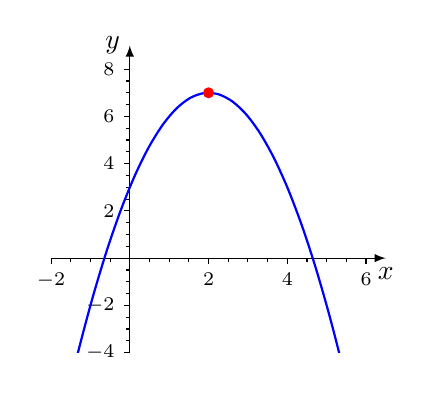
\begin{tikzpicture}[x=5mm,y=3mm,>=latex]
        \draw[thin,black,->] (-2,0) -- (6.5,0) node[below] {$x$};
        \draw[thin,black,->] (0,-4) -- (0,9) node[left] {$y$};
        % ticks:
        \foreach \x in {-2,2,4,6}
        {
          \draw[thin,black] (\x,0) -- (\x,-2pt) node[below] {$\scriptstyle\x$};
        }
        \foreach \x in {-2,-1.5,...,6.2}
        {
          \draw[thin,black] (\x,0) -- (\x,-1.5pt);
        }
        \foreach \y in {-4,-2,2,4,6,8}
        {
          \draw[thin,black] (0,\y) -- (-2pt,\y) node[left] {$\scriptstyle\y$};
        }
        \foreach \y in {-4,-3.5,...,8.2}
        {
          \draw[thin,black] (0,\y) -- (-1.5pt,\y);
        }
        \begin{scope}
          \clip (-2,-4) rectangle (6,8);
          \draw[thick,blue,domain=-2:6.5,smooth] plot (\x,{-1*(\x)^2+4*\x+3});
        \end{scope} 
        \fill[red] (2,7) circle (2pt);
     \end{tikzpicture}
    \end{minipage}
    \hspace*{0.5in}
    \begin{minipage}{0.4\linewidth}
      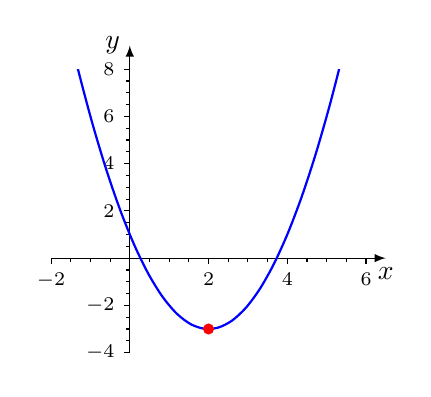
\begin{tikzpicture}[x=5mm,y=3mm,>=latex]
        \draw[thin,black,->] (-2,0) -- (6.5,0) node[below] {$x$};
        \draw[thin,black,->] (0,-4) -- (0,9) node[left] {$y$};
        % ticks:
        \foreach \x in {-2,2,4,6}
        {
          \draw[thin,black] (\x,0) -- (\x,-2pt) node[below] {$\scriptstyle\x$};
        }
        \foreach \x in {-2,-1.5,...,6.2}
        {
          \draw[thin,black] (\x,0) -- (\x,-1.5pt);
        }
        \foreach \y in {-4,-2,2,4,6,8}
        {
          \draw[thin,black] (0,\y) -- (-2pt,\y) node[left] {$\scriptstyle\y$};
        }
        \foreach \y in {-4,-3.5,...,8.2}
        {
          \draw[thin,black] (0,\y) -- (-1.5pt,\y);
        }
        \begin{scope}
          \clip (-2,-4) rectangle (6,8);
          \draw[thick,blue,domain=-2:6.5,smooth] plot (\x,{(\x)^2-4*\x+1});
        \end{scope}
        \fill[red] (2,-3) circle (2pt);
      \end{tikzpicture}
    \end{minipage}
  \end{center}
  \pause
  \bigskip

  What this technique {\blue actually does} is find both maxima and
  minima
  \smallskip

  In Math 34A a problem will have either a maximum {\red or} a
  minimum, {\red but not both}.  So the technique will find what you
  want. In Math 34B you discover how to do problems which have both a
  maximum and a minimum and find out which is which.

}

\frame{
  \frametitle{More Examples}

  \begin{enumerate}
    \setcounter{enumi}{2}
  \item What is the minimum of $f(x)=(x+2)(x+4)+3$?

    \begin{center}
      A $=0$
      \quad 
      B $ = 1$
      \quad 
      C $= 2$
      \quad 
      D $= 3$
      \quad 
      E $= 4$
      \pause
      \quad
    \end{center}
    \alert{Answer:}\ \answer{C}
    \pause
    \bigskip

    \item What is minimum of $f(x)=x^2 + 16 x^{-2}$?
      \begin{center}
        A $=2$
        \quad 
        B $= 4$
        \quad 
        C $= 6$
        \quad 
        D $= 8$
        \quad 
        E $= 16$
        \pause
      \end{center}
      \alert{Answer:}\ \answer{D}
      \pause
      \medskip

      \item Find the value of $x$ which makes $f(x)=-e^x-e^{-2x}$ a
        maximum. 
        \begin{center}
          A $=0$
          \quad 
          B $= \ln(2)$
          \quad 
          C $=-\ln(2)$
          \quad 
          D $= \ln(2)/3$
          \quad 
          E $= \ln(2)/3$
          \pause
        \end{center}
        \medskip
        \alert{Answer:}\ \answer{E}

      \end{enumerate}

}

\section{Word Problems}

\frame{ 
  \frametitle{Word Problem \#1} 

  A ball is thrown into the air. After $t$ seconds the height in
  meters above the ground of the ball is $h(t)=40t-10t^2$. How many
  meters high did the ball go?

  \begin{center}
    A $=2$
    \quad 
    B $= 40-20t$
    \quad 
    C $= 20$
    \quad 
    D $= 40$
    \pause
    \quad
    \fbox{D}
  \end{center}
  \vspace*{2in}

}


\frame{
  \frametitle{Word Problem \#2}

  If an airline sells tickets at a price of $\$200+5x$ each the
  number of tickets it sells is $1000-20x$.  What price should the
  tickets be if the airline wants to get the most money?

  \begin{center}
    A $=5$
    \quad 
    B $= 25$
    \quad 
    C $=175$
    \quad 
    D $= 200$
    \quad 
    E $= 225$
    \pause
    \quad
    \fbox{E}
  \end{center}
  \vspace*{2in}

}

\frame{ 
  \frametitle{Word Problem \#3} 

  A fenced garden with an area of $100\ \text{m}^2$  will be made in
  the shape of a rectangle. It will be surrounded on all four sides by
  a fence. What length and width should be used so the least amount of
  fence is needed? 
  \bigskip
  \pause

  \alert{Approach:}
  \begin{itemize}
  \item[{\blue(1)}] Express the total length of fence in terms of
    \emph{only}\ one variable, either $L = $ length of field, or $W =$
    width of field. This gives a formula for $P=$ (total length of
    fence) involving, say, $W$.
    \pause
    \smallskip

  \item[{\blue(2)}] Find minimum by solving $\dfrac{dP}{dW}=0$.
  \end{itemize}
  \pause
  \bigskip

  Students always find {\blue(1)}\ the hardest part.

  \alert{You}\ have been prepared for this by word problems from chapter 3!
 
  

}






\end{document}


